% !TeX program = lualatex
% !TeX encoding = utf8
% !TeX spellcheck = uk_UA
% !BIB program = bibler

\documentclass[onlytextwidth]{beamer}
\usetheme{Electromagnetism}
\usepackage{Electromagnetism}
\addbibresource{d:/Projects/LaTeX/MyPackage/MyBase.bib}

%============================================================================
\title[Лекції електрики та магнетизму]{\huge\bfseries Електромагнітні хвилі}
\subtitle{Лекції з електрики та магнетизму}
\author{Пономаренко С. М.}
\date{}
%============================================================================
\graphicspath{{pictures/}}
\begin{document}
\begin{frame}[plain]
	\maketitle
\end{frame}


% ============================== Слайд ## ===================================
\begin{frame}{Зміст}{}
	\tableofcontents
\end{frame}
% ===========================================================================



% =================================================
%\begin{frame}{Електромагнітна хвиля}
%\begin{block}{}\justifying
%    	\alert{Електромагнітна хвиля} --- процес розповсюдження коливань електромагнітних полів в просторі.
%\end{block}
%
%\begin{block}{}\justifying
%    	Прикладами \href{https://www.youtube.com/watch?v=QpQhn_yzIb8&t=391s}{електромагнітних хвиль} є світло, радіохвилі, рентгенівські промені,
%    	гамма-промені. Загальні властивості електромагнітних хвиль вивчаються в розділі фізики, що називається класичною електродинамікою, специфічні
%    	--- в інших розділах фізики, таких як радіофізика, оптика, спектроскопія, атомна фізика, ядерна фізика тощо.
%\end{block}
%\end{frame}
% =================================================


% =================================================
%\begin{frame}{Спектр електромагнітних хвиль}
%\begin{block}{}\justifying
%    Електромагнітні хвилі класифікуються за довжиною хвилі $\lambda$ або пов'язаною з нею частотою хвилі.
% \alert{Спектром електромагнітних хвиль} називається смуга частот електромагнітних хвиль, що існують у природі.
%\end{block}
%	\begin{center}
%		\includegraphics[width=\linewidth]{scale.png}
%	\end{center}
%
%	\begin{block}{}\justifying
%		\alert{Світло} (у вузькому сенсі) --- електромагнітні хвилі, що сприймаються людським оком. До таких хвиль належать електромагнітні хвилі в
%		інтервалі частот $7.5 \cdot 10^{14} - 4 \cdot 10^{14}$~Гц, тобто із довжиною хвилі від $390$ до $750$~нм.
%	\end{block}
%
%\end{frame}

% =================================================



% ============================== Слайд ## ===================================
%\begin{frame}{Визначення швидкості світла}
%\framesubtitle<1>{Спостереження Ремера}
%\begin{onlyenv}<1>
%	\begin{center}
%		\includegraphics[width=0.95\linewidth]{ole}
%	\end{center}
%\begin{block}{}\centering\small
%		О́ле Крі́стенсен Ре́мер (дан. Ole Christensen Rømer 1644 -- 1710, Копенгаґен) --- датський астроном, який першим
%		\href{https://www.youtube.com/watch?v=ustuvwHpxYk}{виміряв швидкість світла} (1676).
%\end{block}
%\begin{block}{}\justifying\small
% Вивчаючи затемнення Іо, одного з супутників Юпітера, Ремер виявив, що час між затемненнями змінюється залежно від відстані Землі від Юпітера. Він
% зробив висновок, що ці зміни часу пов'язані з часом, який потрібен світлу для долання додаткової відстані, коли Земля віддаляється від Юпітера. Ремер
% оцінив швидкість світла приблизно в $227\ 000$ км/c, що було першим кількісним вимірюванням цієї величини.
%\end{block}
%\end{onlyenv}
%\begin{onlyenv}<2>
%\framesubtitle<2>{Дослід Фізо}
%\begin{columns}
%	\begin{column}{0.2\linewidth}\centering
%         \includegraphics[width=\linewidth]{Fizo}
%	\end{column}
%	\begin{column}{0.8\linewidth}
%        \begin{block}{}\justifying\small
%            У 1849 році французький фізик Арман Фізо розробив метод, який використовував зубчасте колесо в якості затвора. Світло від джерела проходило
%            через зубчасте колесо, що оберталось і, відбившись від дзеркала, поверталося знову до зубчастого колеса. Знаючи частоту обертання дзеркала і
%            відстань, що проходить світло, Фізо отримав значення близько $313\ 000$~км/с.
%        \end{block}
%	\end{column}
%\end{columns}
%\begin{center}
%\includegraphics[width=\linewidth]{Fizo_exp}
%\end{center}
%\end{onlyenv}
%\end{frame}
% ===========================================================================




% ============================== Слайд ## ===================================
%\begin{frame}{Електродинамічна стала в рівняннях Максвелла}{}\small
%\begin{block}{}\justifying
%    Ще до початку роботи Максвелла над проблемами електромагнетизму, фізикам був відомий експериментальний факт, що якщо виразити величину одного і того
%    ж заряду за допомогою двох різних систем одиниць, а потім знайти відношення отриманих значень, то це відношення --- \alert{електродинамічна стала}
%    $c$ --- матиме розмірність швидкості. Однак більшість учених вважали цей факт незрозумілим фізичним курйозом.
%\end{block}
%
%\begin{block}{}\justifying
%Вебером і Кольраушем було виміряно значення цієї константи, яке виявилось рівним $310\ 740$~км/с.
%\end{block}
%
%\begin{block}{}\justifying
%    Максвелл також провів експерименти з визначення величини цієї константи. Ідея досліду полягала в порівнянні сили електростатичного притягування, що
%    виникає між двома зарядженими дисками із силою відштовхування, що виникає між котушками зі струмом, розміщеними поблизу дисків. Тобто, ніяких
%    вимірювань швидкості світла не проводилось. Максвелл отримав значення  значення $c = 2.88\cdot 10^{10}$~см/с.
%\end{block}
%
%\begin{alertblock}{}\justifying
%    Про історію вимірювання швидкості світла, яку можна назвати <<малою історією фізики>>, і розповідається в книзі \fullcite{Filonovich1983}.
%\end{alertblock}
%
%
%\end{frame}
% ===========================================================================





%% --------------------------------------------------------
\section{Хвильове рівняння}
%% --------------------------------------------------------




% ============================== Слайд ## ===================================
\begin{frame}{Хвильове рівняння}{}\small
	\begin{block}{}\justifying
		Хвиля --- процес поширення коливань в часі та в просторі.
		Хвиля характеризується деякою величиною $u$. Наприклад, у
		випадку хвилі, що поширюється вздовж ланцюжка осциляторів $u$ -- це відхилення від їхнього положення в стані рівноваги.
	\end{block}
	\begin{center}
		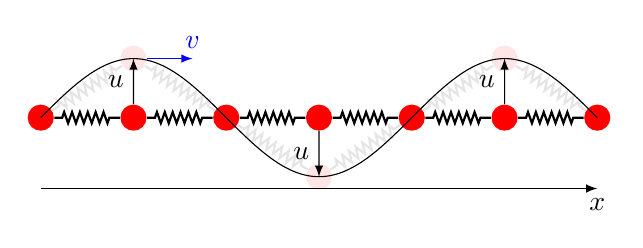
\begin{tikzpicture}[>=latex, scale=0.75,
				bord/.style = {rectangle, fill=blue,
						pattern = north east lines,
						minimum width=5mm, minimum height=25mm,
						yshift=15mm,
						node contents={}},
				mass/.style = {circle, minimum width=2*0.05, fill=red},
				spring/.style = {thick,decorate,decoration={zigzag,
								segment length = 1mm,
								amplitude=0.7mm,
								pre length=1mm, post length=1mm}
					},
			]

			% Начальная точка
			\coordinate (m0) at (0,0);

			% Создаём узлы и соединяем их
			\foreach \i [evaluate=\i as \x using \i*pi/2, evaluate=\i as \y using sin(deg(\x)), count=\j from -1] in {0,...,6} {
					% Создаём массы на синусоиде
					\node[mass] (m\i) at (\x, 0) {};
					\node[mass, opacity=0.1] (um\i) at (\x, \y) {};

					% Рисуем стрелки вверх/вниз для нечётных узлов
					\ifodd\i
						\draw[->] (m\i) --++(0, {(-1)^((\i-1)/2)}) node[left, pos=0.5] {$u$};
					\fi

					% Соединяем соседние узлы пружинами
					\ifnum\i>0
						\draw[spring, opacity=0.1] (um\j) -- (um\i);
						\draw[spring] (m\j) -- (m\i);
					\fi

					\ifnum\i=1
						\draw[->, blue] (um\i) --++(1, 0) node[above] {$\vect{v}$};
					\fi
				}

			% Рисуем синусоиду
			\draw[samples=100, domain=0:6*pi/2, smooth] plot(\x, {sin(deg(\x))});
			\draw[->] (0, -1.2) -- (6*pi/2, -1.2) node[below] {$x$};

		\end{tikzpicture}
	\end{center}
	\begin{block}{}\justifying
		Диференціальне рівняння (яке називається \alert{хвильовим рівнянням}), що описує процес поширення хвилі вздовж осі $x$ має вигляд:
		\begin{equation*}
			\frac{\partial^2 u}{\partial x^2} = \frac1{v^2}\pparttime{u}
		\end{equation*}
		Загальний розв'язок цього рівняння можна подати у вигляді
		\begin{equation*}
			u(x, t) =  \textcolor{red}{f(t - x/v)} + \textcolor{blue}{g(t + x/v)},
		\end{equation*}
		Цей розв'язок є суперпозицією хвиль,  що поширюються як у додатному  напрямку $x$ напрямку (функція $\textcolor{red}{f(t - x/v)}$), так і в
		зворотному (функція $\textcolor{blue}{g(t + x/v)}$).
	\end{block}


\end{frame}
% ===========================================================================





% ============================== Слайд ## ===================================
\begin{frame}{Тривимірний випадок}{}

	\begin{block}{}\justifying
		В тривимірному випадку \alert{хвильове рівняння} має вигляд:
		\begin{equation*}
			\frac{\partial^2 u}{\partial x^2} + \frac{\partial^2 u}{\partial y^2} + \frac{\partial^2 u}{\partial z^2} = \frac1{v^2}\pparttime{u},
		\end{equation*}
		або використовуючи лапласіан: $\nabla^2 = \ddiff{}x + \ddiff{}y +\ddiff{}z$:
		\begin{equation*}
			\tcbhighmath{\nabla^2 u = \frac1{v^2}\pparttime{u}.}
		\end{equation*}
	\end{block}
	\begin{alertblock}{}\centering
		Якщо закони фізики приводять до такого типу рівняння --- то ці закони описують процес поширення хвиль.
	\end{alertblock}
\end{frame}
% ===========================================================================





% ===========================================================================
\begin{frame}{Плоска хвиля}
	\begin{columns}
		\begin{column}{0.59\linewidth}
			\begin{block}{}\justifying
				\alert{Плоскою хвилею} називається хвиля, яка має однакове значення $u$ в усіх точках площин, перпендикулярних до напрямку її поширення.
				Хвиля називається \alert{монохроматичною}, якщо $u$ змінюється з часом за \alert{гармонічним законом} із певною частотою. Для плоскої
				монохроматичної хвилі маємо:
				\begin{equation*}
					u = u_m\cos(\omega t -\vect{k}\vect{r}).
				\end{equation*}
			\end{block}
		\end{column}
		\begin{column}{0.4\linewidth}
			\begin{overprint}
				\onslide<1>
				\begin{center}
					\begin{tikzpicture}[scale=0.6, >=latex]
						\clip (-0.5,-0.5) rectangle (6,5);
						\draw[->] (0, -1) to (0,5) node[below left] {$y$};
						\draw[->] (-1, 0) to (6,0) node[below left] {$x$};
						\foreach \i in {0,1,...,5} {
								‎\draw[domain=-1:30, smooth, variable=\x, blue] plot ({\x}, {-\x + \i}) ;
							}
						\coordinate (K) at (1.5, {-1.5 + 4});
						\coordinate (K1) at (0.5, {-0.5 + 3});
						\coordinate (K2) at (0.6, {-0.6 + 4});
						\coordinate (K3) at (0.6, {-0.6 + 5});
						\draw[->] (0,0) -- node[left=1pt] {$\vect{r}$} (K);
						\draw[->, red, double] (K) -- ++(45:1) node[right] (B) {$\k$};

						\node[font=\tiny, align=center] (k) at (4.5, 2) {Хвильовий вектор\\ --- задає напрям \\ поширення хвилі};
						\draw[-stealth, dash pattern={on 1pt off 0.5pt}] (k.90) to[bend right] (B);

						\node[font=\tiny, align=center] (P) at (4,4.5) {Хвильові\\ площини};
						\draw[-stealth, dash pattern={on 1pt off 0.5pt}] (P.180) coordinate (k1) to[] (K1);
						\draw[-stealth, dash pattern={on 1pt off 0.5pt}] (P.180) coordinate (k1) to[] (K2);
						\draw[-stealth, dash pattern={on 1pt off 0.5pt}] (P.180) coordinate (k1) to[] (K3);
					\end{tikzpicture}
				\end{center}
				\onslide<2>
				\begin{center}
					\includegraphics[width=\linewidth]{plane_wave}
				\end{center}
			\end{overprint}
		\end{column}
	\end{columns}
	\begin{block}{}\justifying
		Для зручності плоску монохроматичну хвилю зручно представити у комплексному вигляді:
		\begin{equation*}
			u = u_m e^{i(\omega t -\vect{k}\vect{r})}.
		\end{equation*}
	\end{block}
	\begin{alertblock}{}\justifying\scriptsize
		Комплексна експоненціальна форма використовується для представлення синусоїдальних хвиль, тому що вона компактно поєднує синус і косинус через
		формулу Ейлера
		\begin{equation*}
			e^{i\theta} = \cos\theta + i\sin\theta,
		\end{equation*}
		спрощує диференціювання та інтегрування (замінюючи операції на множення), дає змогу зручно працювати з фазою і розв'язувати диференціальні рівняння,
		при цьому фізична хвиля залишається дійсною як її реальна частина.
	\end{alertblock}
\end{frame}
% ===========================================================================




% ============================== Слайд ## ===================================
\begin{frame}{Характеристики монохроматичної хвилі}{}
	\begin{block}{Довжина хвилі}\justifying
		Будь-які дві точки, віддалені одна від одної на відстань $\lambda$ коливаються однаково, синхронно: $u(\vect{k}\vect{r}, \omega t) =
			u(\vect{k}\vect{r} + k\lambda , \omega t)$. Величина
		\begin{equation*}
			\lambda = \frac{2\pi}{k}. \quad
            \tikz[]{
                \draw[domain=0:1, smooth, samples=50] plot ({\x}, {0.2*sin(2*pi*\x r)});
                }
		\end{equation*}
		називається \alert{довжиною хвилі}, $\vect{k}$ --- називається \alert{хвильовим вектором}, який напрямлений у
		напрямку
		поширення
		хвилі і перпендикулярний хвильовій поверхні,  $k = |\vect{k}|$ --- називається \alert{хвильовим числом}.
	\end{block}
	\begin{block}{Частота хвилі}\justifying
		Така як $u(\vect{k}\vect{r}, \omega t) =  u(\vect{k}\vect{r}, \omega t + \omega T)$, величина $\omega$ називається коловою \alert{частотою
			хвилі}, а $T$ --- \alert{періодом хвилі}.
	\end{block}
	\begin{block}{Фазова швидкість хвилі}\justifying
		\alert{Фазовою швидкістю хвилі} називається швидкість, з якою поширюється точки з фіксованою фазою:
		\begin{equation*}
			v = \frac{\omega}{k}, \quad \vect{v} = \frac{\omega}{k}\frac{\k}{k}. \quad
            \tikz[>=latex]{
                \draw[domain=0:1, smooth, samples=50] plot ({\x}, {0.2*sin(2*pi*\x r)});
                \draw[->, red] (0.25, 0.2) -- ++(0.5, 0) node[right] {$\vect{v}$};
                }
		\end{equation*}
	\end{block}
\end{frame}
% ===========================================================================






%% --------------------------------------------------------
\section{Електромагнітні хвилі}
%% --------------------------------------------------------





% ============================== Слайд ## ===================================
\begin{frame}{Хвильові рівняння для електромагнітного поля}{Виведення}
	\begin{block}{}\justifying
		Розглянемо електромагнітне поле в однорідній ділянці простору, де немає вільних зарядів і струмів провідності.
	\end{block}
	\begin{columns}
		\begin{column}{0.45\linewidth}
			\begin{block}{}\justifying
				\begin{equation*}
					\begin{cases}
						\Div\Bfield = 0,                                     \\
						\alert<1>{\Rot\Efield = -\frac1c\parttime{\Bfield}}, \\
						\Div\Dfield = 0,                                     \\
						\alert<2>{\Rot\Hfield = \frac1c\parttime{\Dfield}}.
					\end{cases}
				\end{equation*}
				Врахуємо також матеріальні рівняння $\Dfield = \epsilon\Efield$, $\Bfield = \mu\Hfield$.
			\end{block}
		\end{column}
		\quad
		\begin{column}{0.55\linewidth}
			\begin{overprint}
				\onslide<1>
				\begin{block}{}
					До другого рівняння застосуємо операцію $\Rot$:
					\begin{equation*}
						\Rot\Rot\Efield = - \frac1c \parttime{} \Rot\Bfield.
					\end{equation*}
					\begin{equation*}
						\Rot\Rot\Efield =\Grad\Div\Efield - \nabla^2\Efield.
					\end{equation*}
					\begin{equation*}
						- \frac{\mu}c \parttime{}\Rot\Hfield = - \frac{\epsilon\mu}{c^2}\pparttime{\Efield}  .
					\end{equation*}
				\end{block}
				\onslide<2>
				\begin{block}{}
					До четвертого рівняння застосуємо операцію $\Rot$:
					\begin{equation*}
						\Rot\Rot\Hfield = + \frac1c \parttime{} \Rot\Dfield.
					\end{equation*}
					\begin{equation*}
						\Rot\Rot\Hfield =\Grad\Div\Hfield - \nabla^2\Hfield.
					\end{equation*}
					\begin{equation*}
						\frac{\mu}c \parttime{}\Rot\Dfield = - \frac{\epsilon\mu}{c^2}\pparttime{\Hfield}  .
					\end{equation*}
				\end{block}
			\end{overprint}
		\end{column}
	\end{columns}
	\begin{overprint}
		\onslide<1>
		\begin{block}{}
			Приходимо до рівняння для електричного поля:
			\begin{equation*}
				\nabla^2\Efield = \frac{1}{v^2}\pparttime{\Efield}, \quad \text{де}\ v = \frac{c}{\sqrt{\epsilon\mu}}.
			\end{equation*}
		\end{block}
		\onslide<2>
		\begin{block}{}
			Рівняння для магнітного поля:
			\begin{equation*}
				\nabla^2\Hfield = \frac{1}{v^2}\pparttime{\Hfield}, \quad \text{де}\ v = \frac{c}{\sqrt{\epsilon\mu}}.
			\end{equation*}
		\end{block}
	\end{overprint}
\end{frame}
% ===========================================================================



% ============================== Слайд ## ===================================
\begin{frame}{Хвильові рівняння для електромагнітного поля}{}
	\begin{block}{}\justifying
		Рівняння вигляду:
		\begin{equation*}
			\begin{cases}
				\nabla^2\Efield = \frac{1}{v^2}\pparttime{\Efield}, \\
				\nabla^2\Hfield = \frac{1}{v^2}\pparttime{\Hfield}.
			\end{cases}
		\end{equation*}
		називаються хвильовими рівняннями. Вони описують процес поширення величин $\Efield$ та $\Hfield$ у просторі та часі зі швидкістю:
		\begin{equation*}
			v= \frac{c}{\sqrt{\epsilon\mu}}.
		\end{equation*}
		Такий процес називається \alert{електромагнітною хвилею}.
		У вакуумі $\epsilon=\mu=1$, а тому швидкість поширення хвилі буде $v = c =3\cdot10^{10}$~см/с. В середовищі для якого $\epsilon, \mu > 1$, а тому
		швидкість поширення буде меншою ніж у вакуумі $v < c$ на величну:
		\begin{equation*}
			n = \sqrt{\epsilon\mu},
		\end{equation*}
		яка називається \alert{абсолютним показником заломлення середовища}.
	\end{block}
\end{frame}
% ===========================================================================




% =================================================
\begin{frame}[t]{Плоскі електромагнітні хвилі}
	\begin{block}{}
		Розглянемо гармонійні електромагнітні хвилі, які ми представимо в комплексній формі:

		\begin{align*}
			\vect{E} & = \vect{E}_m e^{i(\omega t - \vect{k}\vect{r})} \\
			\vect{H} & = \vect{H}_m e^{i(\omega t - \vect{k}\vect{r})}
		\end{align*}
		Підставимо ці закони в рівняння Максвелла. Диференціальні операції заміняються на:

		\begin{equation*}
			\vect{\nabla} \to -i\vect{k}, \quad \frac{\partial}{\partial t} \to i\omega
		\end{equation*}
		Тоді рівняння Максвелла приймуть вигляд:
		\begin{align*}
			\k\cdot\Efield = 0,
			 & \quad
			\k\cdot\Bfield = 0, \\
			\k\times\Efield    = \frac\omega{c}  \Bfield,
			 & \quad
			-\k\times \Hfield =  \frac\omega{c} \epsilon\Efield
		\end{align*}

	\end{block}
	\begin{onlyenv}<1>
		\begin{block}{}\justifying
			Перші два рівняння показують, що $\Efield\perp\k$ ьа $\Hfield\perp\k$ перпендикулярні напряму поширення, що задається хвильовим векго-
			$\k$. Ця властивість називається \alert{поперечністю електромагнітних хвиль}.
		\end{block}
	\end{onlyenv}
	\begin{onlyenv}<2>
		\begin{block}{}\justifying
			Два інші рівняння дають співвідношення для амплітуд:
			\begin{equation*}
				n E_m = B_m, \quad \sqrt{\epsilon} E_m = \sqrt{\mu}
				H_m
			\end{equation*}
		\end{block}
	\end{onlyenv}
\end{frame}
% ============================== Слайд ## ===================================





%% --------------------------------------------------------
\section{Енергія та вектор Пойнтінга для хвилі}
%% --------------------------------------------------------





% ============================== Слайд ## ===================================
\begin{frame}{Енергія та вектор Пойнтінга для хвилі}{}
	\begin{block}{}\justifying

		Густина енергії (амплітуда)
		\begin{equation*}
			w_m = \frac{\epsilon E_m^2}{8\pi} + \frac{\mu H_m^2}{8\pi}, \quad  \sqrt{\frac{\epsilon}{\mu}} E_m = H_m, \quad w_m = \frac{\epsilon
				E_m^2}{4\pi} = \frac{\mu H_m^2}{4\pi}.
		\end{equation*}
	\end{block}
	\begin{block}{}\justifying
		Вектор Пойнтінга показує напрямок поширення енергії хвилі:
		\begin{equation*}
			\vect{\Pi} = \frac{c}{4\pi}[\Efield\times\Hfield]
		\end{equation*}
		Для хвилі маємо:
		\begin{equation*}
			\vect{\Pi} =  \frac{c^2}{4\pi\epsilon \omega} \Hfield\times\vect{k}\times\Hfield = \frac{c^2}{4\pi\epsilon \omega} H^2 \vect{k} =
			\frac{c}{\omega} \frac{1}{\epsilon\mu}\left( \frac{\mu H^2}{4\pi}\right)   c \vect{k} = w \frac{c}{\sqrt{\epsilon\mu}}
			\frac{\vect{k}}{k}= w
			\vec{v}.
		\end{equation*}
	\end{block}
	\begin{block}{}\justifying\small
		Електромагнітна хвиля --- це електромагнітне поле, що періодично змінюються. У разі високочастотних полів зручно розглядати не миттєві значення
		таких величин, як густина енергії, а значення, усереднені за період коливань. Усереднене в такий спосіб значення вектора Пойнтинга називається
		\alert{інтенсивністю випромінювання}:
		\begin{equation*}
			\left\langle |\vect{\Pi}| \right\rangle = I \propto E^2
		\end{equation*}
	\end{block}
\end{frame}
% ===========================================================================





% ============================== Слайд ## ===================================
\begin{frame}{Плоска монохроматична електромагнітна хвиля}{}
	\begin{center}
		\input{tikz/emwave.tikz}
	\end{center}
\end{frame}
% ===========================================================================




%% --------------------------------------------------------
\subsection{Тиск електромагнітної хвилі}
%% --------------------------------------------------------





% ============================== Слайд ## ===================================
\begin{frame}{Тиск електромагнітної хвилі}{}\small
	\begin{block}{}\justifying
		Електромагнітні хвилі, відбиваючись чи поглинаючись тілами, на які  вони падають, чинять на них тиск. Цей \alert{тиск виникає внаслідок впливу
		магнітного поля хвилі на електричні струми, що збуджуються електричним полем хвилі}.
	\end{block}
	\begin{columns}
		\begin{column}{0.4\linewidth}\centering
			\input{tikz/empresure.tikz}
		\end{column}
		\begin{column}{0.6\linewidth}
			\begin{block}{}\justifying\small
				Електричне поле хвилі збуджує електричний струм густиною $ \vect{j} = \lambda\Efield $. Внаслідок цього на
				об'єму середовища діє сила Ампера:
                \begin{equation*}
                    d\vect{F} = \frac1c[\vect{j}\times\Bfield] dV,
                \end{equation*}
                спрямована убік поширення хвилі. Ця сила викликає тиск електромагнітної хвилі.
			\end{block}
		\end{column}
	\end{columns}
	\begin{block}{}\justifying\small
		\begin{overprint}
			\onslide<1>
            У хвилі магнітне поле $B = nE = \frac{c}{v}E$. Якщо енергія, що падає на поверхню тіла $\Pi dS = wv dS$
            перетворюється на теплову $ jE dV $, то $  wv dS = jEdV$. Отже, сила. що діє на поверхню тіла:
			\begin{equation*}
				dF = \frac1c j B dV = \frac1c j \frac{c}{v}E dV =  \frac1v jE dV = \frac1v wvdS = w dS,
			\end{equation*}
			звідки тиск $ p = \frac{dF}{dS} = w $
			\onslide<2>
			У випадку часткового відбивання, тиск дорівнює
			\begin{equation*}
				p = w (1 + \rho),
			\end{equation*}
			де $ \rho = 0 \ldots 1$ --- коефіцієнт відбивання.
		\end{overprint}
	\end{block}
\end{frame}
% ===========================================================================





% ===========================================================================
\begin{frame}{Тиск світла}{Дослід Лебедєва}\small
	\begin{block}{}\justifying
		Петро Миколайович Лебедєв в 1899 р. вперше виміряв світловий тиск.
	\end{block}
	\begin{columns}
		\begin{column}{0.5\linewidth}
			\begin{block}{}\justifying
				Він підвісив на тонкій нитці коромисло з парою крилець на кінцях:
				поверхня в одного з них була зачорненою, забезпечуючи майже повне поглинання, а в іншого --- дзеркальною, забезпечуючи повне відбивання.
				Підвіс з крильцями утворив чутливі крутильні терези, що поміщаються в посудину, повітря в якому було відкачано.
			\end{block}
		\end{column}
		\begin{column}{0.5\linewidth}\centering
			\includegraphics[width=\linewidth]{LebedevExp}
		\end{column}
	\end{columns}

	\begin{block}{}\justifying
		Світло практично повністю відбивалося від дзеркальної поверхні та його тиск на дзеркальне крильце було вдвічі більше, ніж на зачорнене. Внаслідок цього створювався момент сил, що повертає коромисло. Вимірюючи кут повороту коромисла, можна було виміряти силу, що діяла на крильця, а отже, визначити світловий тиск.
	\end{block}
	{\tiny \url{https://youtu.be/Dr07pTIoue8}}
\end{frame}
% ===========================================================================




% ===========================================================================
\begin{frame}{Тиск світла}{Сонячні вітрила}\small
	\begin{onlyenv}<1>
		\begin{block}{}\justifying
			Сонячне вітрило --- пристрій, що використовує тиск сонячного світла чи лазера на дзеркальну поверхню для приведення в рух космічного апарату.

			\bigskip

			Тиск сонячного світла надзвичайно малий (на Земній орбіті --- близько $5\cdot10^{-6}$~Па) і зменшується пропорційно квадрату відстані від Сонця. В ролі вітрила використовувались сонячні батареї або радіатори системи терморегуляції.
		\end{block}

		\begin{center}
			\includegraphics[width=0.4\linewidth]{Cosmos_solar_sail}
		\end{center}

		{\tiny \url{https://youtu.be/U0_wjnmlmRg}}
	\end{onlyenv}
	\begin{onlyenv}<2>
		\begin{block}{}\justifying
			Вчені з Австралійського національного університету запропонували спосіб запуску для космічного вітрильника до найближчої зірки Альфи Центавра в рамках проекту Breakthrough Starshot. За їх задумом, надати необхідну швидкість апарату допоможе фотонний двигун --- система, що сумарно включає до 100 мільйонів лазерів.
		\end{block}
		\begin{center}
			\includegraphics[width=0.5\linewidth]{Starshot-light-sail_Breakthroughinitiatives}
		\end{center}
		\begin{block}{}\justifying
			Подорож до Альфи Центавра за допомогою звичайних способів переміщення триватиме близько 100 років. Дістатись до Альфи Центавра за допомогою космічного вітрильника на фотонному двигуні передбачається за 20 років зі швидкістю в $ 0.2 c $.
		\end{block}
		{\tiny      \href{https://opg.optica.org/josab/fulltext.cfm?uri=josab-38-5-1477&id=450064}{Journal of the Optical Society of America B}.}
	\end{onlyenv}
	\begin{onlyenv}<3>
		\begin{block}{}\justifying
			Тиск світла відіграє велику роль в астрономічних та атомних явищах. В астрофізиці тиск світла поряд із тиском газу забезпечує стабільність зірок, протидіючи силам гравітації. Дія тиску світла пояснюються деякі форми кометних хвостів. До атомних ефектів відноситься так звана світлова віддача, яку відчуває збуджений атом під час випромінювання фотона.
		\end{block}
		\begin{columns}\centering
			\begin{column}{0.5\linewidth}\centering
				\includegraphics[width=0.75\linewidth]{Star}
			\end{column}
			\begin{column}{0.5\linewidth}\centering
				\includegraphics[width=0.75\linewidth]{Comet}

				\begin{block}{}\tiny\centering
					Товстий білий хвіст комети Гейла-Боппа складається з частинок пилу, і утворюється завдяки тиску світла. Другий, тонкий і блакитний складається з іонів і створюється сонячним вітром.
				\end{block}
			\end{column}
		\end{columns}
	\end{onlyenv}
\end{frame}
% ===========================================================================



%% --------------------------------------------------------
\subsection{Імпульста момент імпульсу електромагнітного поля}
%% --------------------------------------------------------




% ============================== Слайд ## ===================================
\begin{frame}{Імпульс електромагнітного поля}{}
	\begin{block}{}\justifying
		\alert{Поле має енергію}; так само в одиниці об'єму \alert{воно має імпульс}. Оскільки електромагнітна хвиля чинить тиск на речовину, остання
		набуває	певного імпульсу.
	\end{block}

	Для електромагнітної хвилі у вакуумі вектор Пойнтінга.
	\begin{equation*}
		\Pi = w c \Rightarrow \frac{\Pi}{c^2} = \frac{w}{c}.
	\end{equation*}

	З релятивістської механіки $ E^2 = m^2c^4 + p^2c^2 $. Для частинки з нульовою масою (наприклад, фотона) $ m = 0 $, зв'язок енергії та імпульсу:
	\begin{equation*}
		E = p c \Rightarrow  p = \frac{E}{c}.
	\end{equation*}

	Порівнюючи дві останні формули, отримаємо вираз для густини імпульсу:
	\begin{equation*}
		\vect{g} = \frac{\vect{\Pi}}{c^2}, \quad [g] = \frac{\text{дин}\cdot\text{с}}{\text{см}^3}\, \text{(СГС)}
	\end{equation*}
\end{frame}
% ===========================================================================



% ============================== Слайд ## ===================================
\begin{frame}{Імпульс електромагнітної поля}{}
	\begin{block}{}
		Розглянемо такий процес: електромагнітна хвиля поглинається тілом і передає йому свій імпульс.
	\end{block}
	\begin{columns}
		\begin{column}{0.4\linewidth}\centering
			\input{tikz/empresure.tikz}
		\end{column}
		\begin{column}{0.6\linewidth}
			\begin{block}{}\justifying\small
				Електричне поле хвилі збуджує електричний струм густиною $ \vect{j} = \sigma\Efield $ ($ \vect{F} = e\Efield $). Внаслідок цього на
				об'єму середовища діє сила Ампера
				\begin{equation*}
					d\vect{f} = \frac1c[\vect{j}\times\Bfield],
				\end{equation*}
				яка спрямована убік поширення хвилі. Ця сила за час $dt$ змінює імпульс одиниці об'єму тіла на величину:

			\end{block}
		\end{column}
	\end{columns}
	\begin{block}{}\justifying
		\begin{equation*}
			d\vect{g} = \vect{f} dt =  \frac1c[\vect{j}\times\Bfield] dt = \frac{\lambda}{c}[\Efield \times\Bfield]dt =
			\frac{4\pi\lambda}{c^2}\vect{\Pi}dt
			=
			\frac{4\pi\lambda}{c} w \vect{n} dt.
		\end{equation*}
		За той самий час в одиниці об'єму середовища поглинається (передається від поля речовині) енергія:
		\begin{equation*}
			dw = \vect{j}\cdot\Efield dt = \lambda E^2dt = 4\pi\lambda \frac{E^2}{4\pi} dt = 4\pi\lambda w dt
		\end{equation*}
		Звідки $d\vect{g} = \frac{dw}c \vect{n}$, або за весь час дії $\vect{g} = \frac{w}{c} \vect{n} = \frac{\vect{\Pi}}{c^2}$.
	\end{block}
\end{frame}
% ===========================================================================






% ============================== Слайд ## ===================================
\begin{frame}{Момент імпульсу поля}{}\small
	\begin{exampleblock}{Задача}\justifying
		Заряджений циліндричний конденсатор вміщений в зовнішнє однорідне магнітне поле з індукцією $ \Bfield $, що напрямлене вздовж його осі.
		Конденсатор має змогу вільно обертатись навколо своєї осі. Заряд конденсатора $ q $, радіус зовнішньої обкладки $ R $, радіусом внутрішньої
		можна знехтувати.  Маса конденсатора $ m $. Знайдіть вектор моменту імпульсу електромагнітного поля конденсатора. Знайдіть кутову швидкість, з
		якою буде обертатись конденсатор, при вимикання магнітного поля.
	\end{exampleblock}
	\begin{columns}
		\begin{column}{0.25\linewidth}
			\begin{center}
				\begin{tikzpicture}[scale=1.2, >=latex]
					\draw [fill=gray, fill opacity=.25]
					(180:1mm) coordinate (a)
					-- ++(0,-15mm) coordinate (b)
					arc (180:360:1mm and 0.25mm) coordinate (d)
					-- (a -| d) coordinate (c) arc (0:180:1mm and 0.25mm);
					\draw [fill=gray, fill opacity=.25]
					(0,0) coordinate (t) circle (1mm and 0.25mm);
					\draw [densely dashed] (d) arc (0:180:1mm and 0.25mm);

					\draw [thick]
					(180:7.5mm) coordinate (A)
					-- ++(0,-15mm) coordinate (B) %node [midway, right, inner sep=1pt] {$v$}
					arc (180:360:7.5mm and 2.625mm) coordinate (D)
					-- (A -| D) coordinate (C) arc (0:180:7.5mm and 2.625mm);
					\draw [thick]
					(0,0) coordinate (T) circle (7.5mm and 2.625mm);
					\draw [densely dashed] (D) arc (0:180:7.5mm and 2.625mm);

					\foreach[count=\j] \i in {-0.5, 0, 0.5} {
							\draw[blue, <-] (\i,5mm) \ifnum\j=2 node[above] {$\Bfield$} \fi -- ++(0,-25mm);
						}

					\foreach[count=\j] \i in {0, -0.5, -1, -1.5} {
							\draw[red, ->] (1mm,\i) -- ++(6.5mm,0) \ifnum\j=2 node[right] {$ \Efield $}\fi;
							\draw[red, ->] (-1mm,\i) -- ++(-6.5mm,0);
						}

					\draw (0,0) ellipse (1mm and 0.25mm);

					\draw[green!50!black, <-] (0,-0.75) [partial ellipse=110:430:4mm and 1.3mm] node[above, pos=0.2] {$ \vect{\Pi} $};

				\end{tikzpicture}
			\end{center}
		\end{column}
		\begin{column}{0.75\linewidth}
			\begin{block}{}\justifying
				Густина моменту імпульсу поля:
				\begin{equation*}
					\vec{\mathcal{L}} = \vect{r}\times\frac{\vect{\Pi}}{c^2} = \frac{1}{4\pi c} \vect{r}\times \Efield \times \Bfield = - \frac{1}{4\pi c}
					\Bfield (\vect{r}\cdot \Efield)
				\end{equation*}

				Електричне поле :
				\(\displaystyle
				E = \frac{2\lambda}{r} = \frac{2q}{rh}, \quad h - \text{висота циліндра}
				\)

				Модуль вектора імпульсу $ \vect{L} $:
				\begin{equation*}
					L = \iiint\limits_V\mathcal{L} dV = \frac{1}{4\pi c} B \frac{2q}{h} \pi R^2 h = \frac{qBR^2}{2c}, \quad \vect{L} = - \frac{qR^2}{2c}
					\Bfield
				\end{equation*}
			\end{block}
		\end{column}
	\end{columns}
	\begin{block}{}\justifying
		При вимиканні магнітного поля момент імпульсу поля перейде в обертання самого циліндра $ \vect{L} = mR^2\vec\omega
		$, а тому кутова швидкість:
		\(
		\displaystyle	\vec{\omega} = -\frac{q}{2mc}\vect{B}.
		\)
	\end{block}
\end{frame}
% ===========================================================================


\section{Відбивання хвиль від поверхні двох діелектриків}




%% --------------------------------------------------------
\subsection{Поляризація хвиль}
%% --------------------------------------------------------




% ============================== Слайд ## ===================================
\begin{frame}{Поляризація хвиль}{}
	\begin{block}{}\justifying
		\alert{Поляризація хвиль} --- характеристика поперечних хвиль, що описує поведінку вектора величини, яка коливається, у площині, перпендикулярній
		напрямку поширення хвилі.
	\end{block}
	\begin{block}{}\justifying
		Для \alert{$s$-поляризації} напруженість електричного поля електромагнітної хвилі перпендикулярна до площини падіння та паралельна до площини межі
		розділу середовищ.
	\end{block}
	\begin{block}{}\justifying
		\alert{$p$-поляризація} характеризується тим, що
		вектор напруженості електричного поля лежить у площині падіння.
	\end{block}
\end{frame}
% ===========================================================================



%% --------------------------------------------------------
\subsection{Відбивання $s$-поляризованих хвиль від поверхні двох діелектриків}
%% --------------------------------------------------------


% =================================================
\begin{frame}[t]{Відбивання хвиль від поверхні двох діелектриків}%
	{$s$-Поляризована хвиля}
	\begin{columns}
		\begin{column}{0.5\linewidth}
			\begin{center}
				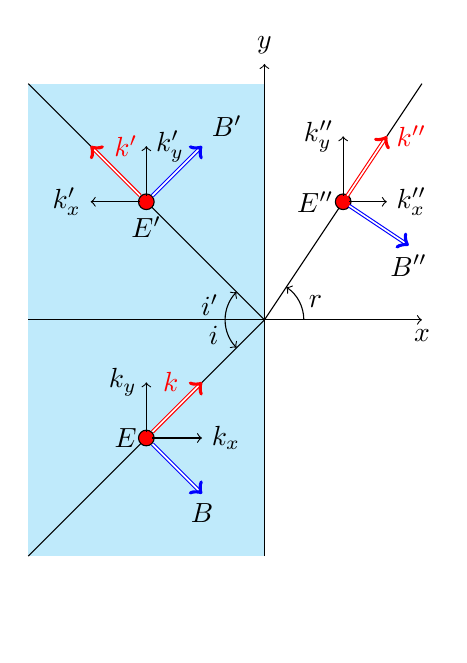
\begin{tikzpicture}[scale=1]
					\fill[cyan!50, opacity=0.5] (-3, -3) rectangle (0, 3);
					\draw[->] (0, -3) to (0,3.25) node[above] {$y$};
					\draw[->] (-3, 0) to (2,0) node[below] {$x$};
					%        \node[circle, draw, anchor=north west, fill=cyan, font=\scriptsize, inner sep=1pt] at (-1, 3) {1};
					%        \node[circle, draw, anchor=north west, fill=cyan, font=\scriptsize, inner sep=1pt] at (1, 3) {2};
					\draw<1-> (-3, -3) -- node[pos = 0.5, inner sep=2pt] (A) {} (0, 0) ;
					\node<1->[circle, draw, inner sep=2pt, fill=red] at (A) {};
					\node<1->[left] at (A) {$\vect{E}$};
					\draw<1->[->, red, double] (A) -- ++(45:1) node[left=5pt] {$\vect{k}$};
					\draw<2->[->] (-0.5, 0) arc (180:225:0.5) node[left, pos=0.5] {$i$};
					\draw<3->[->] (A) -- ++(0:{cos(45)}) node[right] {$k_x$};
					\draw<3->[->] (A) -- ++(90:{sin(45)}) node[left] {$k_y$};
					\draw<4->[blue, ->, double, text=black] (A) -- ++(({atan(3/3) - 90}:1) node[below] {$\vect{B}$};

					\draw<1-> (0, 0) -- node[pos = 0.5, inner sep=2pt] (B) {} (-3, 3);
					\node<1->[circle, draw, inner sep=2pt, fill=red] at (B) {};
					\node<1->[below=2pt] at (B) {$\vect{E}'$};
					\draw<1->[->, red, double] (B) -- ++(135:1) node[right=5pt] {$\vect{k}'$};
					\draw<2->[->] (-0.5, 0) arc (180:135:0.5) node[left, pos=0.5] {$i'$};
					\draw<3->[->] (B) -- ++(0:-{cos(45)}) node[left] {$k'_x$};
					\draw<3->[->] (B) -- ++(90:{sin(45)}) node[right] {$k'_y$};
					\draw<4->[blue, ->, double, text=black] (B) -- ++(({-atan(3/3) + 90}:1) node[above right] {$\vect{B}'$};

					\pgfmathsetmacro{\angle}{atan(3/2)}
					\draw<1-> (0, 0) -- node[pos = 0.5, inner sep=2pt] (C) {} (2, 3);
					\node<1->[circle, draw, inner sep=2pt, fill=red] at (C) {};
					\node<1->[left] at (C) {$\vect{E}''$};
					\draw<1->[->, red, double] (C) -- ++({atan(3/2)}:1) node[right] {$\vect{k}''$};
					\draw<2->[->] (0.5, 0) arc (0:\angle:0.5) node[right, pos=0.5] {$r$};
					\draw<3->[->] (C) -- ++(0:{cos{\angle}}) node[right] {$k''_x$};
					\draw<3->[->] (C) -- ++(90:{sin(\angle)}) node[left] {$k''_y$};
					\draw<4->[blue, ->, double, text=black] (C) -- ++(({\angle - 90}:1) node[below] {$\vect{B}''$};

					\path (0,-4) ++ (1,0);
				\end{tikzpicture}

			\end{center}
		\end{column}
		\begin{column}{0.5\linewidth}
			\only<1-4>
			{
				\begin{block}{}
					Падаюча плоска хвиля:
					\begin{equation*}
						E = E_m e^{i(\omega t - k_xx - k_yy)}
					\end{equation*}

					Відбита плоска хвиля:
					\begin{equation*}
						E' = E'_m e^{i(\omega' t - k'_xx-k'_yy)}
					\end{equation*}

					Заломлена плоска хвиля:
					\begin{equation*}
						E'' = E''_m e^{i(\omega'' t - k''_xx-k''_yy)}
					\end{equation*}
					Гранична умова ($E_{\tau_1} = E_{\tau_2}$), тобто при $x = 0$:
					\begin{equation*}
						E(x=0) + E'(x=0) = E''(x=0),
					\end{equation*}
					або
					\begin{equation*}
						E_m e^{i(\omega t -k_yy)} + E'_m e^{i(\omega' t - k'_yy)} =E''_m e^{i(\omega'' t - k''_yy)}.
					\end{equation*}
				\end{block}
			}
			\only<5>{
				\begin{block}{}
					Продиференціюємо граничні умови
					\begin{enumerate}
						\item 	за часом $t$, отримаємо
						      \begin{equation*}\label{ww}
							      \omega = \omega' = \omega''
						      \end{equation*}
						\item 	за координатою $y$, отримаємо
						      \begin{equation*}\label{ky=ky}
							      k_y = k'_y = k''_y
						      \end{equation*}
					\end{enumerate}
					Тому, гранична умова прийме вигляд:
					\begin{equation*}
						E_m  + E'_m  =E''_m .
					\end{equation*}
					%					З виразу $k = \frac{\omega n}{c}$ і $\omega = \omega' = \omega''$ отримуємо:
					%					\begin{equation*}
					%						\frac{k}{n_1} = \frac{k'}{n_1} = \frac{k''}{n_2}.
					%					\end{equation*}
				\end{block}
			}
			\begin{onlyenv}<6>
				\begin{block}{}\justifying
					З рівняння:
					\begin{equation*}
						%						\frac{k}{n_1} = \frac{k'}{n_1}
						k_y = k'_y
					\end{equation*}
					\begin{equation*}
						k\sin i = k'\sin i'
					\end{equation*}
					\begin{equation*}
						\Rightarrow \frac{\omega n_1}{c} \sin i = \frac{\omega n_1}{c} \sin i'
					\end{equation*}
					%					\[
					%						k_x = - {k'}_x,  \quad k_y = k'_y.
					%					\]
					Звідки випливає закон відбивання, відомий з геометричної оптики:
					\[
						\tcbhighmath{i = i'.}
					\]
				\end{block}
			\end{onlyenv}
			\only<7>{
				\begin{block}{}\justifying
					З рівняння:
					\begin{equation*}
						k'_y = k''_y
					\end{equation*}
					\begin{equation*}
						\frac{\omega n_1}{c}\sin i  = \frac{\omega n_2}{c}\sin r
					\end{equation*}
					Випливає закон заломлення, відомий з геометричної оптики:
					\begin{equation*}
						\tcbhighmath{n_1\sin{i} = n_2\sin{r}}
					\end{equation*}
					або
					\begin{equation*}
						\frac{\sin i}{\sin r} = \frac{n_2}{n_1} = n_{21},
					\end{equation*}
					$n_{21} = \dfrac{n_2}{n_1}$~--- відносний показник заломлення двох середовищ.
				\end{block}
			}
			\only<8>{
				\begin{block}{}\justifying
					Більшість діелектриків не проявляють магнітних властивостей:
					\[
						\mu_1 = \mu_2 \approx 1.
					\]

					Тому, відносний поразник заломлення
					\[
						n_{21} = \frac{n_2}{n_1} = \sqrt{\frac{\epsilon_2}{\epsilon_1}} = \frac{v_1}{v_2}.
					\]
				\end{block}
			}
		\end{column}
	\end{columns}
\end{frame}


% =================================================
\begin{frame}{Формули Френеля для $s$-поляризації}
	\only<1>{Граничні умови для вектора $\Efield$ дають:
		\begin{equation*}
			\tcbhighmath{E_m + E'_m = E''_m}
		\end{equation*}
		а для вектора $\Hfield$ ($H_{\tau_1} = H_{\tau_2}$):
		\begin{equation*}
			H_{0_y} + H'_{0_y} = H''_{0_y} \quad \frac{B_{0_y}}{\mu_1} + \frac{B'_{0_y}}{\mu_1} = \frac{B''_{0_y}}{\mu_2}
		\end{equation*}
		Більшість діелектриків не проявляють магнітних властивостей $\mu_1 = \mu_2 \approx 1$.
		\begin{equation*}
			B_{0_y} + B'_{0_y} = B''_{0_y}
		\end{equation*}
		\[
			\Bfield  = \frac{c}{\omega} \vect{k}\times\Efield  \Rightarrow B_x = \frac{c}{\omega} k_y E, \quad B_y = - \frac{c}{\omega} k_x E, \quad B_z
			= 0.
		\]

		\begin{equation*}
			k_x E_m + k'_x E'_m = k''_x E''_m.
		\end{equation*}
	}
	\only<2>{
		\[
			E_m + E'_m = E''_m
		\]
		\[
			k_xE_m + k'_xE'_m = k''_xE''_m
		\]
		\[
			k_x = -k'_x =\frac{\omega n_1}{c}\cos i, \quad k''_x = +\frac{\omega n_2}{c}\cos r
		\]
		\[
			n_1 E_m \cos i - n_1 E'_m\cos i = n_{2} E''_m \cos r
		\]
		\[
			E_m \cos i - E'_m \cos i = n_{21} (E_m + E'_m) \cos r
		\]
		\begin{equation*}\label{Frenel_s_rl}
			\tcbhighmath{E'_{\perp} = - \frac{\sin(i - r)}{\sin(i + r)} E_{\perp}}
		\end{equation*}
		\begin{equation*}\label{Frenel_s_rr}
			\tcbhighmath{E''_{\perp} = \frac{2\sin r \cos i}{\sin(i + r)} E_{\perp}}
		\end{equation*}
	}
\end{frame}


%% --------------------------------------------------------
\subsection{Відбивання $p$-поляризованих хвиль від поверхні двох діелектриків}
%% --------------------------------------------------------

% =================================================
\begin{frame}[t]{Формули Френеля для $p$-поляризації}%
	\begin{columns}
		\begin{column}{0.5\linewidth}
			\begin{center}
				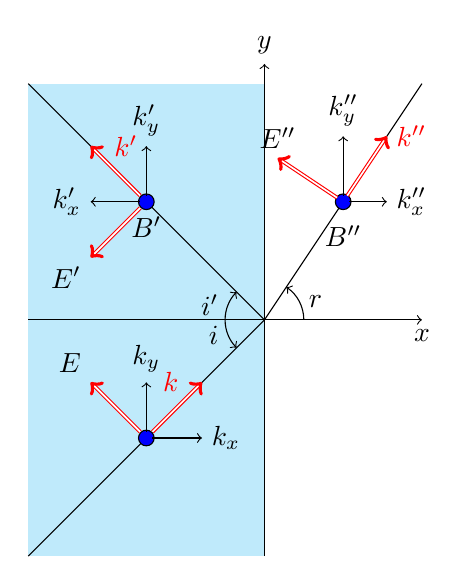
\begin{tikzpicture}[scale=1]
					\fill[cyan!50, opacity=0.5] (-3, -3) rectangle (0, 3);
					\draw[->] (0, -3) to (0,3.25) node[above] {$y$};
					\draw[->] (-3, 0) to (2,0) node[below] {$x$};
					%        \node[circle, draw, anchor=north west, fill=cyan, font=\scriptsize, inner sep=1pt] at (-1, 3) {1};
					%        \node[circle, draw, anchor=north west, fill=cyan, font=\scriptsize, inner sep=1pt] at (1, 3) {2};
					\draw (-3, -3) -- node[pos = 0.5, inner sep=2pt] (A) {} (0, 0) ;
					\node[circle, draw, inner sep=2pt, fill=blue] at (A) {};
					\node[below] at (A) {$\Bfield$};
					\draw[->, red, double] (A) -- ++(45:1) node[left=5pt] {$\vect{k}$};
					\draw[->] (-0.5, 0) arc (180:225:0.5) node[left, pos=0.5] {$i$};
					\draw[->] (A) -- ++(0:{cos(45)}) node[right] {$k_x$};
					\draw[->] (A) -- ++(90:{sin(45)}) node[above] {$k_y$};
					\draw[red, ->, double, text=black] (A) -- ++(({atan(3/3) + 90}:1) node[above left] {$\vect{E}$};

					\draw (0, 0) -- node[pos = 0.5, inner sep=2pt] (B) {} (-3, 3);
					\node[circle, draw, inner sep=2pt, fill=blue] at (B) {};
					\node[below=2pt] at (B) {$\vect{B}'$};
					\draw[->, red, double] (B) -- ++(135:1) node[right=5pt] {$\vect{k}'$};
					\draw[->] (-0.5, 0) arc (180:135:0.5) node[left, pos=0.5] {$i'$};
					\draw[->] (B) -- ++(0:-{cos(45)}) node[left] {$k'_x$};
					\draw[->] (B) -- ++(90:{sin(45)}) node[above] {$k'_y$};
					\draw[red, ->, double, text=black] (B) -- ++(({-atan(3/3) - 90}:1) node[below left] {$\vect{E}'$};

					\pgfmathsetmacro{\angle}{atan(3/2)}
					\draw (0, 0) -- node[pos = 0.5, inner sep=2pt] (C) {} (2, 3);
					\node[circle, draw, inner sep=2pt, fill=blue] at (C) {};
					\node[below=5pt] at (C) {$\vect{B}''$};
					\draw[->, red, double] (C) -- ++({atan(3/2)}:1) node[right] {$\vect{k}''$};
					\draw[->] (0.5, 0) arc (0:\angle:0.5) node[right, pos=0.5] {$r$};
					\draw[->] (C) -- ++(0:{cos{\angle}}) node[right] {$k''_x$};
					\draw[->] (C) -- ++(90:{sin(\angle)}) node[above] {$k''_y$};
					\draw[red, ->, double, text=black] (C) -- ++(({\angle + 90}:1) node[above] {$\vect{E}''$};
				\end{tikzpicture}
			\end{center}
		\end{column}
		\begin{column}{0.5\linewidth}
			\only<1>{
				Граничні умови дають:
				\begin{equation*}
					B_m + B'_m = B''_m
				\end{equation*}
				\begin{equation*}
					E_y + E'_{y_m} = E''_{y_m}
				\end{equation*}
				З рівності  $E_{y_m} = \frac{c k_x}{\epsilon \omega} B$ друга умова приймає вигляд:
				\begin{equation*}
					\frac{k_x}{\epsilon_1}\left( B_m - B'_m\right)  = \frac{k''_x}{\epsilon_2} B''_m
				\end{equation*}
				або
				\begin{equation*}
					n_{21} \cos i \left( B_m - B'_m\right)  = \cos r B''_m
				\end{equation*}
			}
			\only<2>{
				\begin{equation*}\label{Frenel_p_rl}
					\tcbhighmath{E'_{\parallel} = \frac{\tg(i - r)}{\tg(i + r)} E_{\parallel}}
				\end{equation*}
				\begin{equation*}\label{Frenel_p_rr}
					\tcbhighmath{E''_{\parallel} = \frac{2\sin r \cos i}{\sin(i + r)\cos(i - r)} E_{\parallel}}
				\end{equation*}
			}
		\end{column}
	\end{columns}
\end{frame}




%% --------------------------------------------------------
\subsection{Повне внутрішнє відбивання}
%% --------------------------------------------------------




\begin{frame}{Повне внутрішнє відбивання}
	\only<1>{
		Якщо світло йде з матеріалу з показником заломлення з оптично більш густого в оптично менш густе $n_2 < n_1$, то згідно закону відбивання
		$\dfrac{\sin i}{\sin r} = \frac{n_2}{n_1} = n_{21} < 1 \Rightarrow i < r$.
		\begin{columns}
			\begin{column}{0.4\linewidth}
				\begin{center}
					\includegraphics[width=\textwidth]{totrefr}
				\end{center}
			\end{column}
			\begin{column}{0.6\linewidth}
				Коли кут заломлення $r = 90^\circ$ при при куті падіння $i = i_b$, який називається граничним і визначається рівністю:
				\begin{multline*}
					\sin i_b = \frac{n_2}{n_1} = n_{21}, \text{або}\, n\sin i_b = 1,\\ \text{де}\, n = \frac{n_1}{n_2} > 1
				\end{multline*}
				виникає \href{https://www.youtube.com/watch?v=HN37Jz8DHYg}{повне внутрішнє відбивання}.
			\end{column}
		\end{columns}
		Що відбувається із заломленим променем при $i > i_b$, тобто при кутах падіння. що більші ніж граничний кут?
	}
	\only<2>{
	\[
		\Efield'' = \Efield''_m e^{i(\omega t - {k''_x} - {k''_y})}
	\]
	\[
		\frac{k^2}{n^2}  = {k''_x}^2 + {k''_y}^2
	\]
	\[
		\sin i =\frac{k_y}{k}, \quad k_y = {k''_y}
	\]
	\[
		{k''_x}^2 =  \frac{k^2}{n^2} (1 - n^2\sin^2 i)  = \frac{\omega^2}{c^2}(1 - n^2\sin^2 i)
	\]
	Оскільки при $i > i_b$, $1 - n^2\sin^2 i < 0$,

	то ${k''_x}^2 < 0 \Rightarrow k''_x = i K, \quad K =   \frac{\omega^2}{c^2}(1 - n^2\sin^2 i) > 0$.

	Тоді розв'язок рівнянь Максвелла буде мати вигляд:

	\[
		\Efield'' = \Efield''_me^{-Kx} e^{i(\omega t - {k''_y})}
	\]
	\alert{В $2$-му середовищі буде поле при $i > i_b$, однак його амплітуда буде експоненційно спадати вздовж $x$}.
	}
	%	\only<3>{
	%
	%		$K$ за порядком величини дорівнює $\frac{\omega}{c}$, дорівнює довжині хвилі світла в вакуумі $\lambda_0$.
	%
	%		Коли світло повністю відбивається від внутрішньої поверхні скло --- повітря, то в повітрі виникають поля, але вони виходять за границю розділу
	%		межі на відстань порядку довжини хвилі світла. Тепер нам зрозуміло, як потрібно відповідати на таке запитання: якщо світлова хвиля у склі падає
	%		на поверхню під досить великим кутом, вона повністю відбивається; якщо ж присунути до поверхні інший шматок скла (так що поверхня фактично
	%		зникає), то світло буде проходити. В який момент відбувається цей перехід? Адже, напевно, має існувати неперервний перехід від повного
	%		відбивання до повного його відсутності! Відповідь, полягає у тому, що прошарок повітря настільки малий, що експоненційний <<хвіст>>
	%		$\Efield_0e^{-Kx}$ хвилі в повітрі має ще відчутну величину у другому шматку скла, він <<трясе>> електрони і породжує нову хвилю.
	%
	%		Для звичайного світла цей ефект проходження можна спостерігати, тільки якщо щілина дуже мала (порядку довжини хвилі, тобто $10^{5}$ см), але для
	%		$3$ сантиметрових хвиль він демонструється дуже легко.
	%
	%		\href{https://www.feynmanlectures.caltech.edu/II_33.html}{The Feynman Lectures on Physics, Volume II, 33 Reflection from Surfaces}
	%	}
\end{frame}


\end{document}
